\documentclass{beamer}

\usepackage{amsmath,amssymb}
\usepackage{tikz}
\usepackage{graphicx}
\usepackage{multicol}
\usepackage[per-mode=fraction]{siunitx}

\usetheme{Boadilla}
\usecolortheme{orchid}

\usetikzlibrary{calc}

\tikzset{>=stealth}


\title{PHYS2350: Forces}
\author{Dr. Wolf}
\date{Fall 2024}

\begin{document}

\begin{frame}
  \titlepage
\end{frame}

\begin{frame}
  {Group discussion:}
    \begin{block}{What is a force?}
      \uncover<2->{
        \begin{itemize}
          \item A push or a pull (it is a \textit{vector})
          \item An interaction between two things
        \end{itemize}
      }
    \end{block}

    \uncover<3->{
      \begin{block}{How do you remember good ideas?}
        \uncover<4->{
          Develop a notation to describe forces
        \begin{itemize}
          \item<4-> Write force as a vector thing: $\vec{F}$
          \item<5-> Indicate that there are two interacting entities:
          $\vec{F}_{\text{Book},\text{Table}}$
        \end{itemize}
        }
      \end{block}
    }
\end{frame}

\begin{frame}
  {Group discussion:}
  \begin{block}
    {What kinds of forces are there?}  \uncover<2->{
      \begin{enumerate}
        \item Contact Forces \uncover<3->{
          \begin{itemize}
            \item Friction
            \item ``Normal'' force
            \item Tension
            \item Air resistance
            \item Spring force
          \end{itemize}
        }
        \item Non-contact forces \uncover<4->{
          \begin{itemize}
            \item Gravity/Weight
            \item Electric Force
            \item Magnetic Force
            \item Nuclear Force
          \end{itemize}
        }
      \end{enumerate}
    }
  \end{block}
  \uncover<5->{ Force notation:
    \[
      \vec{F}^{(\text{type})}_{A,B}
    \]
  }
\end{frame}

\begin{frame}
  {Rules for good Free-Body diagrams}
  \begin{enumerate}
    \item Use our force notation to label each force
    \[
      \vec{F}^{(\text{type})}_{A,B}
    \]
    \item Draw a vector in the \textit{direction} that the force is going in. Don't worry about
    the length. 
    \item Put the tail of the force vector on the object.
  \end{enumerate}
\end{frame}

\begin{frame}
  {Part \textrm{I}}
  Free body diagram for box being pushed/pulled by Pam and Chris
  \begin{center}
    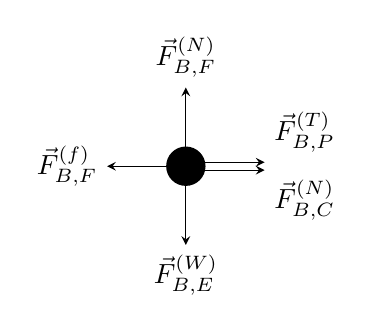
\begin{tikzpicture}
      \coordinate (O) at (0,0);
      \fill (O) circle (0.25);
      \draw[->] ($(O) + (0,0.05)$) -- ++(1,0) node [above right]
           {$\vec{F}^{(T)}_{B,P}$};
      \draw[->] ($(O) + (0,-0.05)$) -- ++(1,0) node [below right]
           {$\vec{F}^{(N)}_{B,C}$};
      \draw[->] (O) -- ++(0,1) node [above] {$\vec{F}^{(N)}_{B,F}$};
      \draw[->] (O) -- ++(-1,0) node [left] {$\vec{F}^{(f)}_{B,F}$};
      \draw[->] (O) -- ++(0,-1) node [below] {$\vec{F}^{(W)}_{B,E}$};
    \end{tikzpicture}
  \end{center}
  Symbol key:
  \begin{columns}
    \begin{column}{0.5\textwidth}
      \begin{itemize}
        \item P = Pam
        \item C = Chris
        \item F = Floor
      \end{itemize}      
    \end{column}
    \begin{column}{0.5\textwidth}
      \begin{itemize}
        \item B = Block
        \item E = Earth
      \end{itemize}      
    \end{column}
  \end{columns}
\end{frame}

\begin{frame}
  {Part \textrm{II}} Free body diagram for book on table
  \begin{center}
    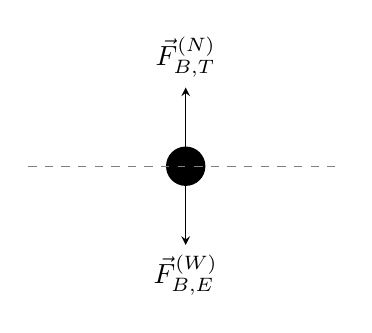
\begin{tikzpicture}
      \coordinate (O) at (0,0); \fill (O) circle (0.25);
      \draw[black!50,dashed] (-2,0) -- (2,0);

      \draw[->] (O) -- ++(0,1) node [above] {$\vec{F}^{(N)}_{B,T}$};

      \draw[->] (O) -- ++(0,-1) node [below] {$\vec{F}^{(W)}_{B,E}$};
    \end{tikzpicture}
  \end{center}
  Symbol key:
  \begin{itemize}
    \item B = Book
    \item T = Table
    \item E = Earth
  \end{itemize}
\end{frame}

\begin{frame}
  {Part \textrm{II}} Free body diagram for books on table
  \begin{center}
    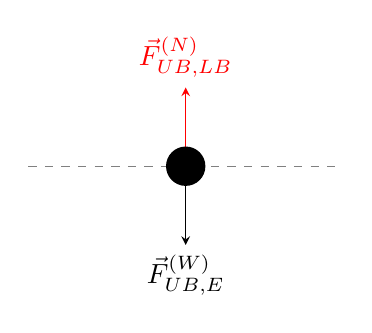
\begin{tikzpicture}
      \coordinate (O) at (0,0);
      \draw[black!50,dashed] (-2,0) -- (2,0);

      \draw[->,red] (O) -- ++(0,1) node [above] {$\vec{F}^{(N)}_{UB,LB}$};

      \draw[->] (O) -- ++(0,-1) node [below] {$\vec{F}^{(W)}_{UB,E}$};
      \fill (O) circle (0.25);
    \end{tikzpicture} \hspace{1cm}
    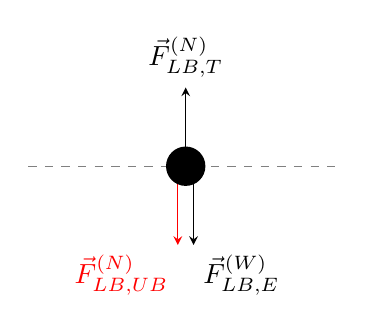
\begin{tikzpicture}
      \coordinate (O) at (0,0); 
      \draw[black!50,dashed] (-2,0) -- (2,0);

      \draw[->] (O) -- ++(0,1) node [above] {$\vec{F}^{(N)}_{LB,T}$};
      \draw[->,red] ($(O)+(-0.1,0)$) -- ++(0,-1) node [below left] {$\vec{F}^{(N)}_{LB,UB}$};

      \draw[->] ($(O)+(0.1,0)$) -- ++(0,-1) node [below right] {$\vec{F}^{(W)}_{LB,E}$};
      \fill (O) circle (0.25);
    \end{tikzpicture}
  \end{center}
  Symbol key:
  \begin{itemize}
    \item UB = Upper Book
    \item LB = Lower Book
    \item T = Table
    \item E = Earth
  \end{itemize}
\end{frame}

\begin{frame}
  {Part \textrm{III}}
  Why did I make these vectors \textcolor{red}{red}?
  \begin{center}
    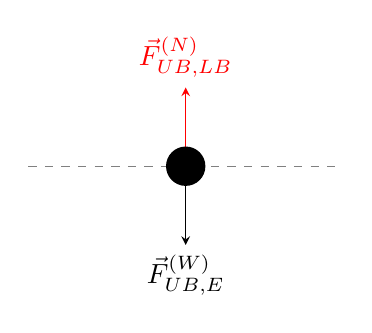
\begin{tikzpicture}
      \coordinate (O) at (0,0);
      \draw[black!50,dashed] (-2,0) -- (2,0);

      \draw[->,red] (O) -- ++(0,1) node [above] {$\vec{F}^{(N)}_{UB,LB}$};

      \draw[->] (O) -- ++(0,-1) node [below] {$\vec{F}^{(W)}_{UB,E}$};
      \fill (O) circle (0.25);
    \end{tikzpicture} \hspace{1cm}
    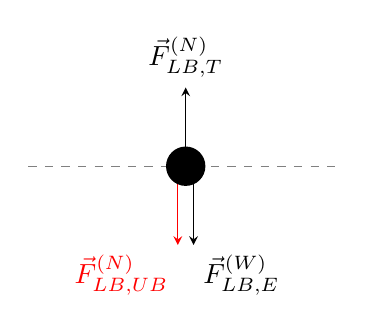
\begin{tikzpicture}
      \coordinate (O) at (0,0); 
      \draw[black!50,dashed] (-2,0) -- (2,0);

      \draw[->] (O) -- ++(0,1) node [above] {$\vec{F}^{(N)}_{LB,T}$};
      \draw[->,red] ($(O)+(-0.1,0)$) -- ++(0,-1) node [below left] {$\vec{F}^{(N)}_{LB,UB}$};

      \draw[->] ($(O)+(0.1,0)$) -- ++(0,-1) node [below right] {$\vec{F}^{(W)}_{LB,E}$};
      \fill (O) circle (0.25);
    \end{tikzpicture}
  \end{center}
  \begin{columns}
    \begin{column}{0.4\textwidth}
      Symbol key:
      \begin{itemize}
        \item UB = Upper Book
        \item LB = Lower Book
        \item T = Table
        \item E = Earth
      \end{itemize}
    \end{column}
    \begin{column}{0.6\textwidth}
      \begin{block}
        {Newton's 3\textsuperscript{rd} Law}
        How does our notation make identifying 3rd law pairs easy?
      \end{block}
    \end{column}
  \end{columns}
\end{frame}


\end{document}